%% 
%% Copyright 2007-2020 Elsevier Ltd
%% 
%% This file is part of the 'Elsarticle Bundle'.
%% ---------------------------------------------
%% 
%% It may be distributed under the conditions of the LaTeX Project Public
%% License, either version 1.2 of this license or (at your option) any
%% later version.  The latest version of this license is in
%%    http://www.latex-project.org/lppl.txt
%% and version 1.2 or later is part of all distributions of LaTeX
%% version 1999/12/01 or later.
%% 
%% The list of all files belonging to the 'Elsarticle Bundle' is
%% given in the file `manifest.txt'.
%% 
%% Template article for Elsevier's document class `elsarticle'
%% with harvard style bibliographic references

%\documentclass[preprint,12pt,authoryear]{elsarticle}

%% Use the option review to obtain double line spacing
%% \documentclass[authoryear,preprint,review,12pt]{elsarticle}

%% Use the options 1p,twocolumn; 3p; 3p,twocolumn; 5p; or 5p,twocolumn
%% for a journal layout:
%% \documentclass[final,1p,times,authoryear]{elsarticle}
%% \documentclass[final,1p,times,twocolumn,authoryear]{elsarticle}
%% \documentclass[final,3p,times,authoryear]{elsarticle}
%% \documentclass[final,3p,times,twocolumn,authoryear]{elsarticle}
%% \documentclass[final,5p,times,authoryear]{elsarticle}
\documentclass[final,5p,times,twocolumn]{elsarticle}
\biboptions{number, sort&compress}

%% For including figures, graphicx.sty has been loaded in
%% elsarticle.cls. If you prefer to use the old commands
%% please give \usepackage{epsfig}

%% The amssymb package provides various useful mathematical symbols
\usepackage{amssymb}
\usepackage{lipsum}
\usepackage{fancyhdr}
\usepackage{multirow}
%% The amsthm package provides extended theorem environments
%% \usepackage{amsthm}

%% The lineno packages adds line numbers. Start line numbering with
%% \begin{linenumbers}, end it with \end{linenumbers}. Or switch it on
%% for the whole article with \linenumbers.
%%\usepackage{lineno}

%% You might want to define your own abbreviated commands for common used terms, e.g.:
\newcommand{\kms}{km\,s$^{-1}$}
\newcommand{\msun}{$M_\odot}
\usepackage{setspace}

\usepackage{xcolor,colortbl}

\newcommand{\mc}[2]{\multicolumn{#1}{c}{#2}}
\definecolor{Gray}{gray}{0.90}

\newcolumntype{a}{>{\columncolor{Gray}}c}
\newcolumntype{b}{>{\columncolor{white}}c}


\journal{LAP}

\begin{document}
\begin{spacing}{1.125}

\begin{frontmatter}
%% Title, authors and addresses

%% use the tnoteref command within \title for footnotes;
%% use the tnotetext command for theassociated footnote;
%% use the fnref command within \author or \affiliation for footnotes;
%% use the fntext command for theassociated footnote;
%% use the corref command within \author for corresponding author footnotes;
%% use the cortext command for theassociated footnote;
%% use the ead command for the email address,
%% and the form \ead[url] for the home page:
%% \title{Title\tnoteref{label1}}
%% \tnotetext[label1]{}
%% \author{Name\corref{cor1}\fnref{label2}}
%% \ead{email address}
%% \ead[url]{home page}
%% \fntext[label2]{}
%% \cortext[cor1]{}
%% \affiliation{organization={},
%%            addressline={}, 
%%            city={},
%%            postcode={}, 
%%            state={},
%%            country={}}
%% \fntext[label3]{}

\title{Benchmarking Dynamatic against modern HLS tools}

%% use optional labels to link authors explicitly to addresses:
%% \author[label1,label2]{}
%% \affiliation[label1]{organization={},
%%             addressline={},
%%             city={},
%%             postcode={},
%%             state={},
%%             country={}}
%%
%% \affiliation[label2]{organization={},
%%             addressline={},
%%             city={},
%%             postcode={},
%%             state={},
%%             country={}}

\author[1]{Elija-Angelo Dirren}
\author[1]{under the supervision of Andrea Guerrieri}
\affiliation[1]{organization={Ecole Polytechnique Fédérale de Lausanne (EPFL)},%Department and Organization
            addressline={School of Computer and Communication Sciences}, 
            city={Lausanne},
            country={Switzerland}}

\begin{abstract}
%% Text of abstract
High level synthesis tools present a more agile approach for designing digital systems than classical workflows. Dynamatic, an open-source HLS tool using dynamic scheduling, provides a novel approach to generate circuits capable of overcoming irregular or general-purpose code which would normally bring statically scheduled HLS tools to their knees. The goal of this project is to define a common ground on which these tools with differing architectures can be
compared, in the form of a set of benchmarks. Our results show that Dynamatic is indeed vastly superior when confronted with designs prone to create imbalances in the distribution of the workload accross components, but is outperformed when confronted with regular and nested code, when compared against Xilinx' Vitis. In contrast with Intel HLS however, Dynamatic is far ahead in every aspect, even though Intel boasts using dynamic scheduling themselves, with some peculiar behavior.
\end{abstract}

%%Graphical abstract
%\begin{graphicalabstract}
%\includegraphics{grabs}
%\end{graphicalabstract}

%%Research highlights
%\begin{highlights}
%\item Research highlight 1
%\item Research highlight 2
%\end{highlights}

\begin{keyword}
%% keywords here, in the form: keyword \sep keyword, up to a maximum of 6 keywords
high-level synthesis \sep dynamic scheduling \sep dataflow

%% PACS codes here, in the form: \PACS code \sep code

%% MSC codes here, in the form: \MSC code \sep code
%% or \MSC[2008] code \sep code (2000 is the default)

\end{keyword}


\end{frontmatter}

%\tableofcontents

%% \linenumbers

%% main text

\section{INTRODUCTION}
There is no doubt that \textit{high level synthesis} (HLS) tools present a viable alternative to more classic design procedures, foregoing the need of designing circuits with RTL languages in favor of using high-level languages such as C and C++ to accelerate design workflows. This allows for a behavior-driven approach, making designing circuits more available to software-inclined users. When generating the design, most common industry-standard HLS tools use a \textit{static schedule}, where the point in time at which each operation is executed is decided during synthesis. This approach functions well for operations ordered in a regular manner, when the workload is equally distributed across all of the components, but can incur large performance penalties when confronted with irregular code rich in logical branches, due to the schedule's conservative nature \cite{dataflow_circs}.

An alternative is to use a \textit{dynamic schedule}, where the point in time where an operation is executed is determined during circuit runtime. This allows a design to adapt to irregularly distributed workloads, and improve performance over static schedules as a consequence. Dynamatic is an open-source HLS framework which utilizes dynamic scheduling to improve performance and allows for more general-use code to be translated into efficient circuits \cite{dyn_tut}.

This report outlines how Dynamatic compares to its commercial counterparts, Vitis and Intel HLS, provided by Xilinx and Intel respectively, and the procedures involved to allow for meaningful and comparable results.

\section{TOOLS TO BE COMPARED}
%%\label{}
In this section, we establish some context for each of the tools used to draw comparisons in the project. The tools chosen to be compared against Dynamatic are developed by the two biggest FPGA manufacturers, Xilinx and Intel. Both companies have their own dedicated HLS tool, optimized for their respective FPGA architecture and toolchain.

\subsection{Dynamatic}
\begin{figure*}
	\centering 
	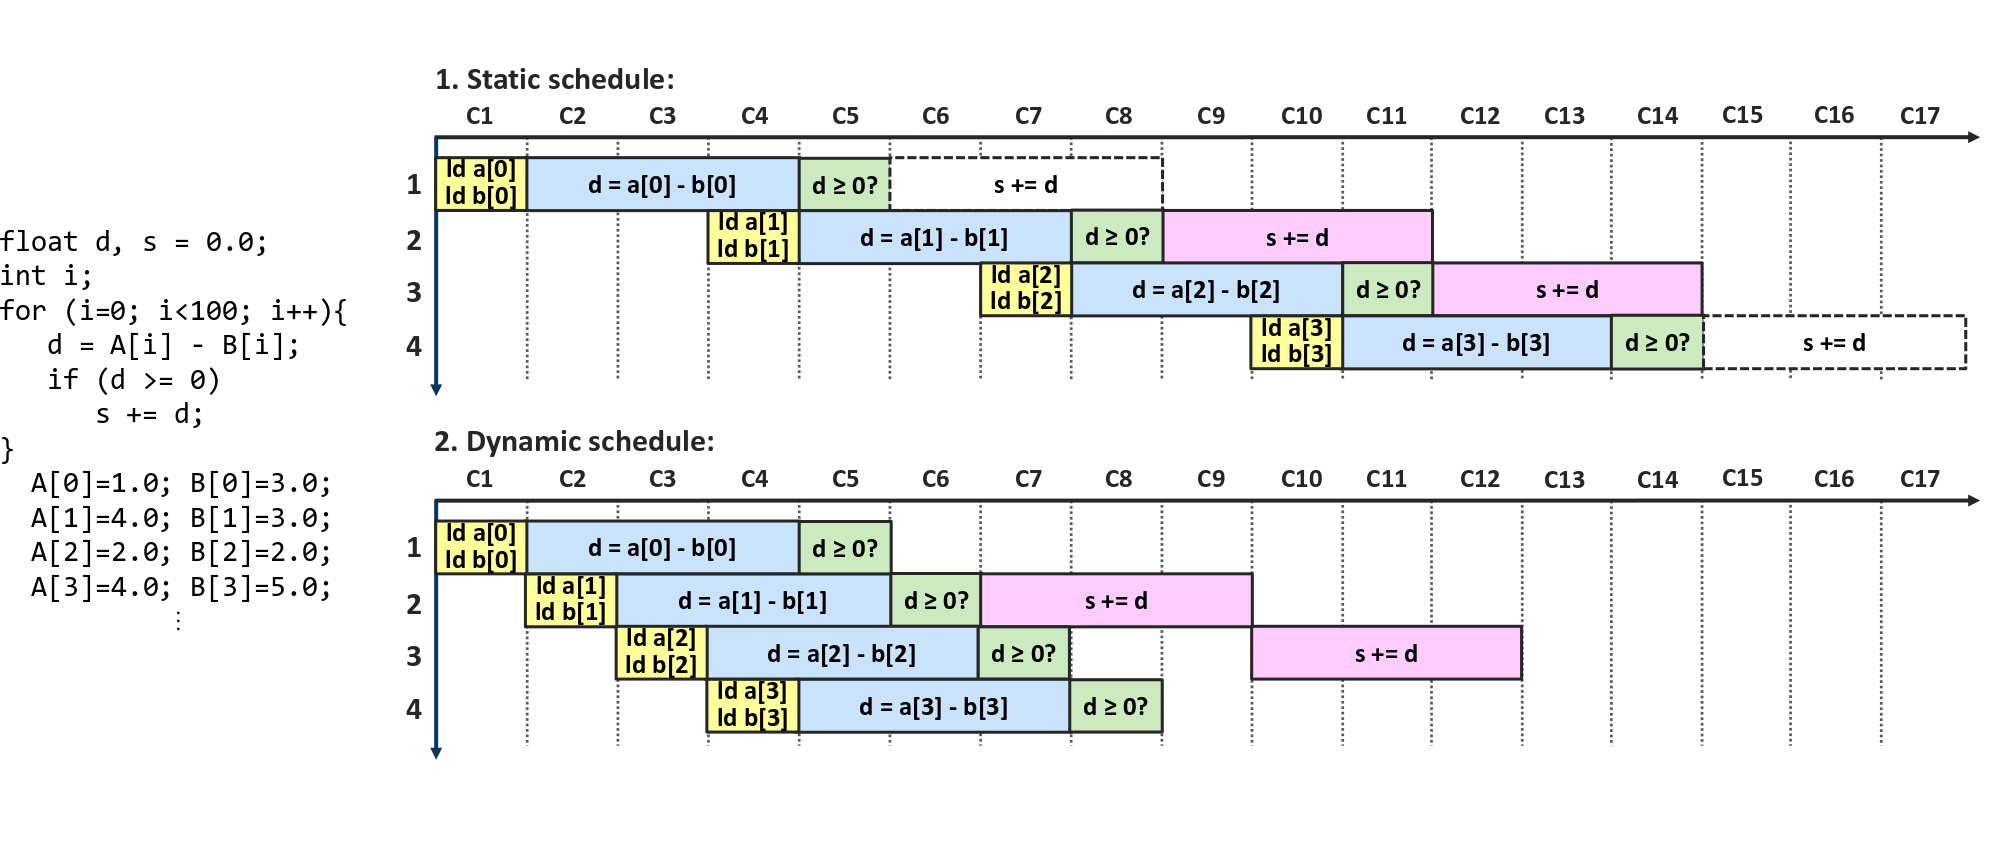
\includegraphics[width=6.2in\textwidth]{schedules-cropped.png}	
	\caption{Difference between a static, conservative schedule and a dynamic schedule} 
	\label{fig_mom0}%
\end{figure*}

Dynamatic is an academic HLS compiler specifically designed to make use of dynamic scheduling to improve performance on irreglar and more general-use code. The approach to generating the circuits is different from a statically scheduled tool, since it uses handshakes between individual components to signal when an operation is ready to receive data. This is beneficial for designs with logical conditions. For instance, if a branch is not taken, instead of effectively losing the space a static schedule would reserve in the pipeline, a 'ready' signal would propagate from the branch up to the previous operation, signalling that it is ready to receive the next batch of data, and skipping ahead to the next iteration of the loop. This is effective for reducing the \textit{initiation interval} (II) of a loop inside one of these designs, reducing the number of cycles between each consecutive iteration of the loop. Figure 1 illustrates a visual example of the difference between a static and a dynamic schedule, where one can note the difference in II between the two scheduling approaches, as well as the lost space the conservative approach of the static schedule entails in the pipeline \cite{dyn_tut}.

\subsection{Vitis}
The Vitis HLS tool (formerly Vivado HLS) is Xilinx' own HLS tool. As such, it is optimized for Xilinx FPGAs, and interfaces with the Vivado design suite to synthesize onto its boards. Vitis uses static scheduling to generate its circuit, so we expect it to perform less than average when confronted with designs with an imbalance in workload across components \cite{vitis_hls}.

\subsection{Intel HLS}
The Intel HLS tool is Intel's own HLS tool. It is optimized for Intel FPGAs, and interfaces with the Quartus design software to build onto its boards. Unlike Vitis, according to Intel, the tool uses dynamic scheduling through the means of handshaking, just like Dynamatic \cite{intel_hls}\cite{intel_dyn_sched}. If this information reveals itself to be true, we can expect Intel HLS to do comparatively well when confronted with designs rich in logical conditions, where the workload across components can be unbalanced.

\section{TARGETS}

This section describes which target architectures have been chosen. Since Xilinx and Intel are each optimized to their own architectures, we compare Dynamatic's results on each platform to their respective commercial HLS tool.

\subsection{Xilinx target}

Dynamatic, by default, targets a Xilinx Kintex-7 device, and the tool's latest optimizations have been built on this platform \cite{dyn_tut}.

\subsection{Intel target}

Dynamatic also supports a Cyclone V board as one of its targets. Unlike the Kintex-7 target however, Intel targets did not receive the latest of Dynamatic's optimizations like improved buffer placement, fast-token delivery and LSQ sizing \cite{dyn_repository}.

\section{EXPERIMENTAL SETUP}

\begin{table*}[t]
\centering
\begin{tabular}{l l l} 
 \hline
 \textbf{Category} & \textbf{Benchmark} & \textbf{Description} \\
 \hline
 \hline
 \textbf{Category 1} & getTanh &  CORDIC-based hyperbolic tangent computation \\
 & triangular & Triangular matrix-multiply \\
 & fir & Ordinary finite impulse response (FIR) filter \\
 \hline
 \textbf{Category 2} & histogram & Computes the histogram of an array \\
 & jacobi\_1d & 1-D Jacobi stencil computation  \\
 & atax & Matrix Transpose and Vector Multiplication \\
 & bicg & Subkernel of the BiCGStab linear solver \\
  \hline
 \textbf{Category 3} & if\_loop\_1 & Conditional loop summing if over a threshold, with input values multiplied by a factor \\
  & if\_loop\_2 & Conditional loop summing if over a threshold \\
  & if\_loop\_3 & Conditional loop: integer division if input a is bigger than input b \\
  \hline
  \textbf{Category 4} & stencil2d & 2-dimensional Stencil computation \\
  & gaussian & Ordinary Gaussian filter \\
  & 2mm & 2 Matrix Multiplications (D=A\cdot B; E=C\cdot D)\\
  & 3mm & 3 Matrix Multiplications (E=A\cdot B; F=C\cdot D; G=E\cdot F) \\
  & covariance & Covariance Computation \\
  & matvec & Matrix Vector product \\
  \hline
\end{tabular}
\caption{Description of the benchmarks}
\label{Table1}
\end{table*}

This section describes the methods used to compare the performance of the tools.

\subsection{Benchmarks}

There are a total of 16 benchmarks, retrieved from two previous papers which themselves originate from the PolyBench\\C 3.2 test suite, and from Dynamatic's regression testing examples \cite{dyn_repository}\cite{unleash}\cite{sttq}\cite{polybench}. These benchmarks can be divided into four distinct categories, being:
\begin{enumerate}[1.]
\item \textbf{Regular memory accesses:} benchmarks of the most basic nature, simple loops with low levels of nesting with few to no data dependencies
\item \textbf{Regular memory accesses with data dependencies:} loops or chains of loops with data dependencies
\item \textbf{Conditional writes:} loops containing conditions, which trigger depending on the inputs on a per-iteration basis
\item \textbf{Deep loop nesting:} loops or chains of loops with multiple levels of nesting
\end{enumerate}

In particular for benchmarks of the third category, due to the nature of dynamic scheduling, Dynamatic's performance depends on the inputs we supply to those particular benchmarks. As such, we define the best, worst, and average performance as when 0\%, 100\% and 50\% of the conditions trigger, respectively \cite{dataflow_circs}. Note that all benchmarks are supplied with random values which satisfy these conditions, but consistent between tools. A description for each benchmark is illustrated in Table 1.

\subsection{Dynamatic vs. Vitis}

Dynamatic and Vitis have almost identical syntax requirements for their input C++ code, meaning that the benchmark source files have very few differences. Additionally, some of Dynamatic's internal arithmetic components interface with Vivado's IP libraries directly; this is expected since Dynamatic was mainly designed to be used in conjunction with Vivado. To generate the data, we start by running the benchmark in Dynamatic with the included regression testing framework. We can then retrieve the generated RTL and import it into Vivado to get the resource utilization and maximum frequency. During the regression testing, Dynamatic also generates a test bench which we can launch in ModelSim to get timing info such as the II and total cycle count. Occasionally, the test-bench will fail to compile due to a misconfigured signal width in the testbench and the single argument component, but this is easily fixed by correcting the values manually. For Vitis, we separate the benchmark component from the test bench, and run the synthesis. The generated report already contains all resource usage and timing information, but to tie the data with what we retrieved from Dynamatic, we run the generated RTL in Vivado to get actual resource usage \cite{dyn_tut}\cite{vivado}\cite{modelsim}.

\subsection{Dynamatic vs. Intel HLS}

Dynamatic and Intel HLS have differing syntax for their input C++ code. One key difference is inputs to the circuit; what could be easily defined as a simple array in Dynamatic will trigger Intel HLS into defining the inputs through the target's I/O, which hugely affects read and write latencies. The first idea to circumvent this issue was to force Intel HLS to use the FPGA's on-board memory, but this causes issues with our test-bench. For instance, in Intel's syntax, on-board memory can only be initialized by a component synthesized onto the board, which would skew our obtained results in one way or another. If we synthesize an initialization component to the board, we jeopardize the resource usage metrics; if we implement the initialization into the component under verification, the total cycle count would be skewed. The final solution to this problem was using memory interfaces as input vectors, which mimic the behavior of on-board memory but are still able to be targeted by the test-bench.

As mentioned above, some of Dynamatic's components reference Vivado's IP libraries \cite{dyn_repository}. Since we need to use Quartus to be able to build our designs on Intel components, this requires us to retrieve some of Vivado's components and add them to the VHDL source files. In addition, Vivado's and Quartus' VHDL parsers have minute differences, requiring us to adapt some of the existing arithmetic unit components to be able to synthesize them with Quartus. Another concession are space issues caused by Dynamatic's LSQs. For benchmarks with deep loop nesting (\textit{2mm} and \textit{3mm} specifically) with a large amount of inputs, the LSQs are too large to be fitted to the Cyclone V board. As such, the LSQs have been disabled for these particular benchmarks to be able to fit them on the FPGA.

Once these issues are resolved, we run the benchmarks on Dynamatic with the specified Cyclone V target. We then modify the arithmetic and elastic components in the generated RTL, and import them into Quartus, set all pins to virtual (similar to Vivado's \textit{out of context} mode) and run the synthesis to retrieve the resource usage and maximum frequency. Just like with Vitis, we then run the ModelSim simulation to retrieve the total cycle count and II. For Intel HLS, we adapt the benchmarks to use memory interfaces instead of plain arrays as inputs, and run the software verification and co-simulation. We then open the generated project files in Quartus to retrieve the resource usage and maximum frequency, and view the wave graph artifacts in ModelSim to determine total cycle count and II. Note that Intel HLS generates a report file containing this data, but we do not make use of it since it would eliminate the common points between the two tools. The report does however supply us with the per-iteration schedule of the circuit, as well as the dataflow graph, similar to the artifacts generated by Dynamatic \cite{intel_hls}\cite{modelsim}\cite{quartus}.

\subsection{Buffer placement and characterization}

One obvious flaw of the comparisons between Dynamatic and Intel HLS are the advanced features like improved buffer placement and fast-token delivery missing for the Cyclone V target. In fact, these optimizations have been implemented after the delay and latency files for the Cyclone V target have been created \cite{dyn_repository}. This results in below-average performance for Dynamatic when building to this target. To generate the delay list, we use a \textit{characterization script}, which retrieves timing data for most of the internal components Dynamatic uses to generate the design with. The script iterates over the different connectors of each components (data, valid, read), fixes the width to a set value ranging from 1 bit to 64, runs the component through a hardware synthesizer for a specific target, and fetches the delay for that particular component-connector-width combination. When this is done with all of the components required for the elastic pass, Dynamatic can then use that data to optimize the buffer placement for the design for the target \cite{buffers}. Since this hasn't been done for the Cyclone V target before, we adapted an existing script running for Vivado to use Quartus instead. This required a lot of adjustment, and still lacks a lot of the functionality of the original script due to the library discrepancies between Vivado and Quartus which Dynamatic's components depend on, but serves as a rudimentary implementation of the improved buffer placement scheme, adapted to our Cyclone V target.

\section{RESULTS}

This section discusses the results obtained from the benchmarks. 

\begin{table*}[t]
\centering
\resizebox{\textwidth}{!}{%
\def\arraystretch{1.2}%
\begin{tabular}{l a a b b a a b b a a} 
 \hline
 \textbf{Bench-} & \multicolumn{2}{a}{\textbf{FF}} & \multicolumn{2}{b}{\textbf{II}} & \multicolumn{2}{a}{\textbf{Av. cycle count}} & \multicolumn{2}{b}{\textbf{Fmax [MHz]}} & \multicolumn{2}{a}{\textbf{Av. execution time [µs]}}\\
 \textbf{mark} & Vitis & Dynamatic & Vitis & Dynamatic & Vitis & Dynamatic & Vitis & Dynamatic & Vitis & Dynamatic \\
 \hline
 \hline
 getTanh & 1051 & 4265 & 18 & 1 & 18005 & 6025 & 290 & 104 & 62.17 & 57.98 \\
 triangular & 1058 & 5058 & 6 & 1 & 30892 & 9895 & 299 & 129 & 103.46 & 76.98 \\
 fir & 455 & 508 & 1 & 1 & 1007 & 1008 & 299 & 249 & 3.37 & 4.04 \\
 \hline
 histogram & 383 & 4365 & 2 & 1 & 2005 & 1016 & 355 & 152 & 5.64 & 6.68\\
 jacobi\_1d & 334 & 3267 & 2 & 1 & 907 & 1174 & 360 & 165 & 2.52 & 7.11\\
 atax & 12361 & 3656 & 34 & 6 & 691 & 3009 & 299 & 162 & 2.31 & 18.62\\
 bicg & 13593 & 868 & 30 & 1 & 917 & 1389 & 299 & 188 & 3.07 & 7.39 \\
 \hline
 if\_loop\_1 & 136 & 797 & 1 & 1 & 102 & 109 & 290 & 176 & 0.35 & 0.62 \\
 if\_loop\_2 & 101 & 751 & 1 & 1 & 101 & 105 & 290 & 168 & 0.35 & 0.63 \\
 if\_loop\_3 & 2483 & 1751 & 35 & 2 & 3503 & 1903 & 275 & 172 & 12.73 & 11.06 \\
 \hline
 stencil2d & 3242 & 1155 & 5 & 13 & 3937 & 11041 & 276 & 177 & 14.28 & 62.27 \\
 gaussian & 816 & 3336 & 2 & 1 & 6002 & 17452 & 299 & 152 & 20.10 & 114.52 \\
 2mm & 7378 & 8133 & 5 & 2 & 1026 & 5599 & 293 & 139 & 3.50 & 40.40 \\
 3mm & 8357 & 10117 & 5 & 3 & 1023 & 8388 & 298 & 142 & 3.43 & 59.07 \\
 covariance & 14102 & 1294 & 32 & 2 & 10390 & 122341 & 232 & 236 & 44.77 & 519.34 \\
 matvec & 9644 & 641 & 15 & 31 & 481 & 938 & 299 & 219 & 1.61 & 4.29 \\
 \hline
\end{tabular}}
\caption{Dynamatic vs. Vitis - results}
\label{Table1}
\end{table*}

\begin{figure}
	\centering 
	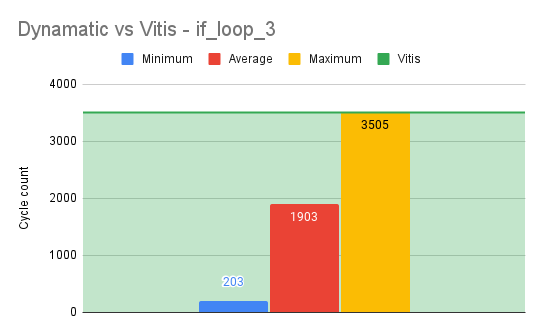
\includegraphics[width=0.45\textwidth]{vitis_if_loop_cycles.png}	
	\caption{Dynamatic vs. Vitis - if\_loop\_3 - cycle count} 
	\label{fig_mom0}%
\end{figure}

\begin{figure}
	\centering 
	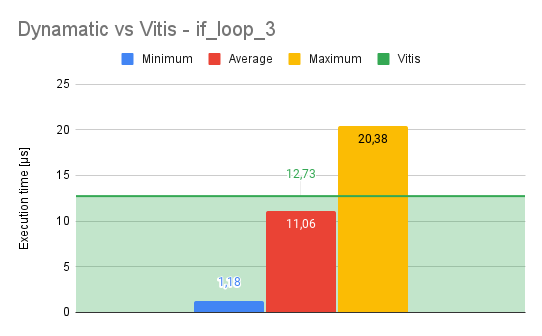
\includegraphics[width=0.45\textwidth]{vitis_if_loop_runtime.png}	
	\caption{Dynamatic vs. Vitis - if\_loop\_3 - execution time} 
	\label{fig_mom0}%
\end{figure}



\subsection{Dynamatic vs. Vitis}

Table 2 illustrates the results obtained when comparing Dynamatic with Vitis. At a first glance, Dynamatic's scheduling is very effective at keeping the II at a minimum for almost all of the benchmarks. For regular memory accesses (category 1), the average cycle count correlates with the II. Due to the simple nature of the loops, having a lower II is crucial for achieving good performance in this respect. For regular accesses with data dependencies (category 2), static schedules can optimize memory accesses to improve performance. This becomes especially apparent when looking at deeply nested loops (category 4), where further optimizations such as loop flattening and loop merging can improve performance for nested and chained loops respectively \cite{vitis_ug}, and dynamic scheduling falls short.

For conditional loops (category 3) however, we can observe the main advantage of dynamic scheduling; the \textit{if\_loop\_3} benchmark in particular is tailored to maximize the performance difference between static and dynamic schedules, where the condition in the loop contains a long-latency division operation which substantially reduces the cycle count each time the condition is false. In figures 2 and 3, we can see that the performance, as expected, varies depending on the inputs supplied, where the worst-case cycle count matches those of the static schedule. In the best and average cases however, the advantages clearly become apparent. The only observable setbacks in terms of cycle count are due to the increased overhead created by the handshakes.

Finally, Dynamatic's resource usage tends to be higher than average due to the use of LSQs which are area-intensive. Benchmarks which do not use LSQs such as \textit{atax} remain in the ballpark of what Vitis achieves.

\begin{table*}[t]
\centering
\resizebox{\textwidth}{!}{%
\def\arraystretch{1.2}%
\begin{tabular}{l a a b b a a b b a a} 
 \hline
 \textbf{Bench-} & \multicolumn{2}{a}{\textbf{FF}} & \multicolumn{2}{b}{\textbf{II}} & \multicolumn{2}{a}{\textbf{Av. cycle count}} & \multicolumn{2}{b}{\textbf{Fmax [MHz]}} & \multicolumn{2}{a}{\textbf{Av. execution time [µs]}}\\
 \textbf{mark} & Intel HLS & Dynamatic & Intel HLS & Dynamatic & Intel HLS & Dynamatic & Intel HLS & Dynamatic & Intel HLS & Dynamatic \\
 \hline
 \hline
 getTanh & 4387 & 5029 & 115 & 10 & 48008 & 10006 & 195 & 88 & 246 & 114 \\
 triangular & 5693 & 5999 & 69 & 1 & 348581 & 10407 & 194 & 77 & 1797 & 135 \\
 fir & 1799 & 742 & 1 & 3 & 2023 & 3009 & 199 & 186 & 10 & 16 \\
 \hline
 histogram & 3437 & 4596 & 98 & 3 & 31010 & 3009 & 165 & 85 & 188 & 35\\
 jacobi\_1d & 7811 & 3952 & 66 & 1 & 12988 & 1780 & 152 & 97 & 85 & 26\\
 atax & 9987 & 5210 & 69 & 3 & 11651 & 2486 & 149 & 89 & 78 & 28\\
 bicg & 10207 & 3917 & 69 & 3 & 24521 & 2789 & 155 & 90 & 158 & 31 \\
 \hline
 if\_loop\_1 & 1168 & 764 & 1 & 3 & 120 & 311 & 226 & 186 & 0.53 & 1.67 \\
 if\_loop\_2 & 1135 & 944 & 1 & 3 & 119 & 307 & 216 & 166 & 0.55 & 1.85 \\
 if\_loop\_3 & 3756 & 3323 & 9 & 5 & 959 & 1903 & 170 & 61 & 5.64 & 31.20 \\
 \hline
 stencil2d & 5032 & 1477 & 1 & 3 & 51947 & 30695 & 175 & 144 & 297 & 213 \\
 gaussian & 7714 & 5419 & 69 & 1 & 71261 & 9140 & 169 & 79 & 422 & 116 \\
 2mm & 6882 & 4110 & 1 & 1 & 7270 & 6872 & 179 & 94 & 41 & 73 \\
 3mm & 10662 & 3250 & 1 & 1 & 17480 & 10300 & 176 & 110 & 99 & 94 \\
 covariance & 6921 & 2060 & 1 & 3 & 59739 & 58709 & 166 & 122 & 360 & 481 \\
 matvec & 2823 & 954 & 1 & 3 & 2855 & 2797 & 175 & 128 & 16 & 22 \\
 \hline
\end{tabular}}
\caption{Dynamatic vs. Intel HLS (non-characterized) - results}
\label{Table1}
\end{table*}

\begin{figure}
	\centering 
	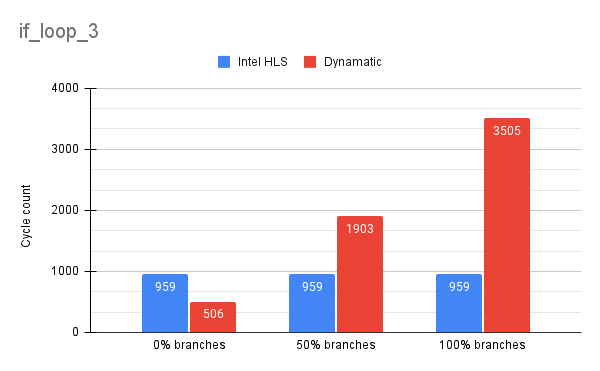
\includegraphics[width=0.45\textwidth]{intel_if_loop_cycles.png}	
	\caption{Dynamatic vs. Intel HLS - if\_loop\_3 (non-characterized) - cycle count} 
	\label{fig_mom0}%
\end{figure}

\begin{figure}
	\centering 
	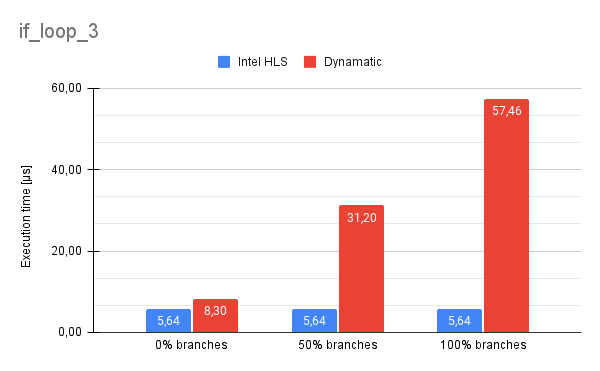
\includegraphics[width=0.45\textwidth]{intel_if_loop_runtime.png}	
	\caption{Dynamatic vs. Intel HLS - if\_loop\_3 (non-characterized) - execution time} 
	\label{fig_mom0}%
\end{figure}



\subsection{Dynamatic vs. Intel HLS}

Table 3 illustrates the results obtained when comparing Dynamatic with Intel HLS. Once again, Dynamatic does well for keeping the II at a minimum and outperforms Intel HLS in almost all categories, except for the conditional loops (category 3). This would suggest that, if Intel HLS really does use dynamic scheduling, it outperforms Dynamatic in this respect. This hypothesis is further supported by the poor performance Intel HLS achieves for deeply nested loops (category 4), which are difficult to optimize without merging of flattening loops, techniques which are typical for statically scheduled tools to compensate for their drawbacks in respect to dynamic schedules \cite{viv_dyn_bench}.

When looking at figures 4 and 5 however, we see an unusual pattern: Intel HLS' cycle count and runtime are not affected by the inputs supplied to the design. If we inspect the RTL generated by Intel HLS, we can see that the valid and stall signals for handshaking are very well generated into the design. If we look into the wave graph however, even though handshaking takes place, no performance gains are achieved, even with inputs which cause none of the branches in the loop. For instance, when looking at the schedule generated in the report file of the benchmark, it indicates that the empty space created in the schedule when no branch takes place is not utilized, and the select component tasked with retrieving the value resulting from the condition, whether it takes place or not, is \textit{statically} scheduled to start after the number of cycles equal to the latency of the division operation. This puts Intel HLS into a very awkward position where it only has the drawbacks of dynamic scheduling, without harnessing any of its benefits.

Finally, due to the very rudimentary state of the characterization script, only a handful of benchmarks can be generated correctly by Dynamatic with the improved buffer placement scheme. Figures 6 and 7 plot the cycle counts and execution time of the original delay files against the characterized variant. The only noticeable difference can be observed in the best case scenario, along with a reduction of the II from 5 to 2, reducing the runtime to a lower value than Intel HLS, even though the design runs at only a third of the frequency.

\subsection{Further considerations}

These results, although complete, still leave some questions unanswered. For instance, when comparing Dynamatic to Intel HLS, it is still limited in capabilities, even against an odd optimization scheme. In addition, the Cyclone V target, although proven as a platform, is at this point in time, thirteen years old \cite{cyc_v}. One can only wonder how Dynamatic would compare to Intel HLS' performance on newer, larger, and faster FPGAs, especially when using the latest optimizations in buffer placement and fast-token delivery.

\begin{figure}
	\centering 
	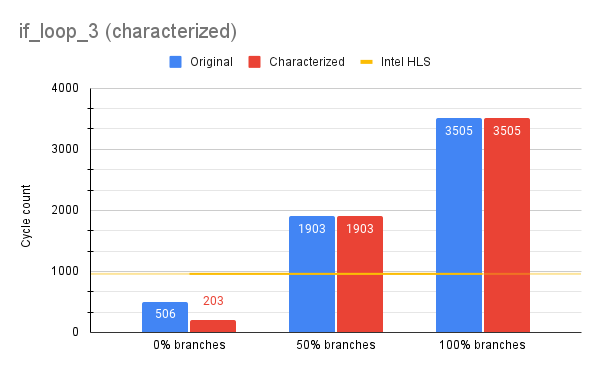
\includegraphics[width=0.45\textwidth]{dyn_char_cycles.png}	
	\caption{Dynamatic vs. Intel HLS - if\_loop\_3 (characterized) - cycle count} 
	\label{fig_mom0}%
\end{figure}

\begin{figure}
	\centering 
	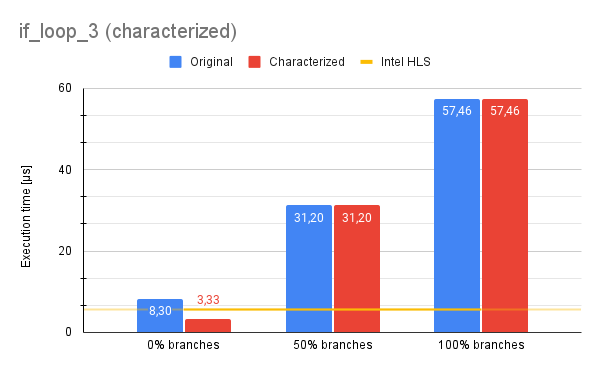
\includegraphics[width=0.45\textwidth]{dyn_char_runtime.png}	
	\caption{Dynamatic vs. Intel HLS - if\_loop\_3 (characterized) - execution time} 
	\label{fig_mom0}%
\end{figure}

\section{CONCLUSIONS}
%%\label{}
Dynamatic, thanks to its dynamic scheduling, stands its ground against industry-standard HLS tools when faced with irregular and general-purpose code. Although static schedules provide ample performance when dealing with regular and easily optimizable designs, dynamic token-based designs capable of adapting their behavior to the supplied inputs provide us with an open-source alternative, supporting a wider range of use cases and designs. The drawbacks of dynamic scheduling are however still apparent, especially for well established commercial HLS tools like Xilinx' Vitis.


\section*{Acknowledgements}
Thanks to Andrea Guerrieri for supervising this semester project, and his contributions by providing valuable insight on the matter. Further thanks go to Carmine Rizzi, member of the DYNAMO group at ETH Zurich for providing the foundation for the characterization script.

%% The Appendices part is started with the command \appendix;
%% appendix sections are then done as normal sections

%% \label{}

%% If you have bibdatabase file and want bibtex to generate the
%% bibitems, please use
%%

%% else use the following coding to input the bibitems directly in the
%% TeX file.

\begin{thebibliography}{00}

%% \bibitem[Author(year)]{label}
%% For example:

\bibitem[]{dataflow_circs} L. Josipović, A. Guerrieri, and P. Ienne. From C/C++ Code to High-Performance Dataflow Circuits. In \textit{IEEE TRANSACTIONS ON COMPUTER-AIDED DESIGN OF INTEGRATED CIRCUITS AND SYSTEMS}, Volume 41, pages 2142-2155, July 2022.
\bibitem[]{dyn_tut} L. Josipović, A. Guerrieri, and P. Ienne. Dynamatic: From C/C++ to Dynamically Scheduled Circuits. Invited tutorial. In \textit{In Proceedings of the 28th ACM/SIGDA International Symposium on Field Programmable Gate Arrays}, Seaside, Calif., February 2020.
\bibitem[]{vitis_hls} Xilinx Inc. \textit{Vivado High-Level Synthesis}.
\bibitem[]{intel_hls} Intel Corporation. \textit{Intel High Level Synthesis Compiler }.
\bibitem[]{intel_dyn_sched} Intel Corporation. Dynamic scheduling. \textit{https://www.intel.com/content/www/us/en/docs/programmable/683152/21-3/dynamic-scheduling.html}.
\bibitem[]{dyn_repository} Dynamatic. \textit{https://github.com/lana555/dynamatic}.
\bibitem[]{unleash} A. Elakhras, A. Guerrieri, L. Josipovi´c and P. Ienne. Unleashing Parallelism in Elastic Circuits with Faster Token Delivery. \textit{32nd International Conference on Field Programmable Logic and Applications}, Belfast, United Kingdom, Sep. 2022.
\bibitem[]{sttq} A. Elakhras,  R. Sawhney, A. Guerrieri, L. Josipovi´c and P. Ienne. Straight to the Queue: Fast Load-Store Queue Allocation in Dataflow Circuits. In \textit{Proceedings of the 31st ACM/SIGDA International Symposium on Field Programmable Gate Arrays}, Monterey, Calif., February 2023. 
\bibitem[]{vivado} Xilinx Inc. \textit{Vivado Design Suite}.
\bibitem[]{modelsim} Mentor Graphics. \textit{ModelSim}.
\bibitem[]{quartus} Intel Corporation. \textit{Intel Quartus Prime Design Software}.
\bibitem[]{buffers} L. Josipović, S. Sheikhha, A. Guerrieri, P. Ienne, and J. Cortadella. Buffer placement and sizing for high-performance dataflow circuits. In \textit{ACM Transactions on Reconfigurable Technology and Systems (TRETS)}. 15(1):1–32, November 2021.
\bibitem[]{vitis_ug} Xilinx Inc. \textit{Vitis High-Level Synthesis User Guide}.
\bibitem[]{viv_dyn_bench} J. Cheng, L. Josipović, G. Constantinides and J. Wickerson. Dynamic Inter-Block Scheduling for HLS. \textit{32nd International Conference on Field Programmable Logic and Applications}, Belfast, United Kingdom, September 2022.
\bibitem[]{cyc_v} Intel Corporation. \textit{Cyclone V E FPGA}.
\bibitem[]{polybench} The Polyhedral Benchmark suite. \textit{https://web.cse.ohio-state.edu/~pouchet.2/software/polybench/}.

\end{thebibliography}

\end{spacing}
\end{document}

\endinput
%%
%% End of file `elsarticle-template-harv.tex'.
